\chapter{生成式設計}
運用電腦輔助系統的創造工具,利用軟體設計出所需的3D模型,輸入的參數或製作、預期要求,將成品利用電腦算法,強大的運算會模擬許多所有可能性及排列,並產生多個解決方案。\\

\begin{figure}[hbt!]
\center
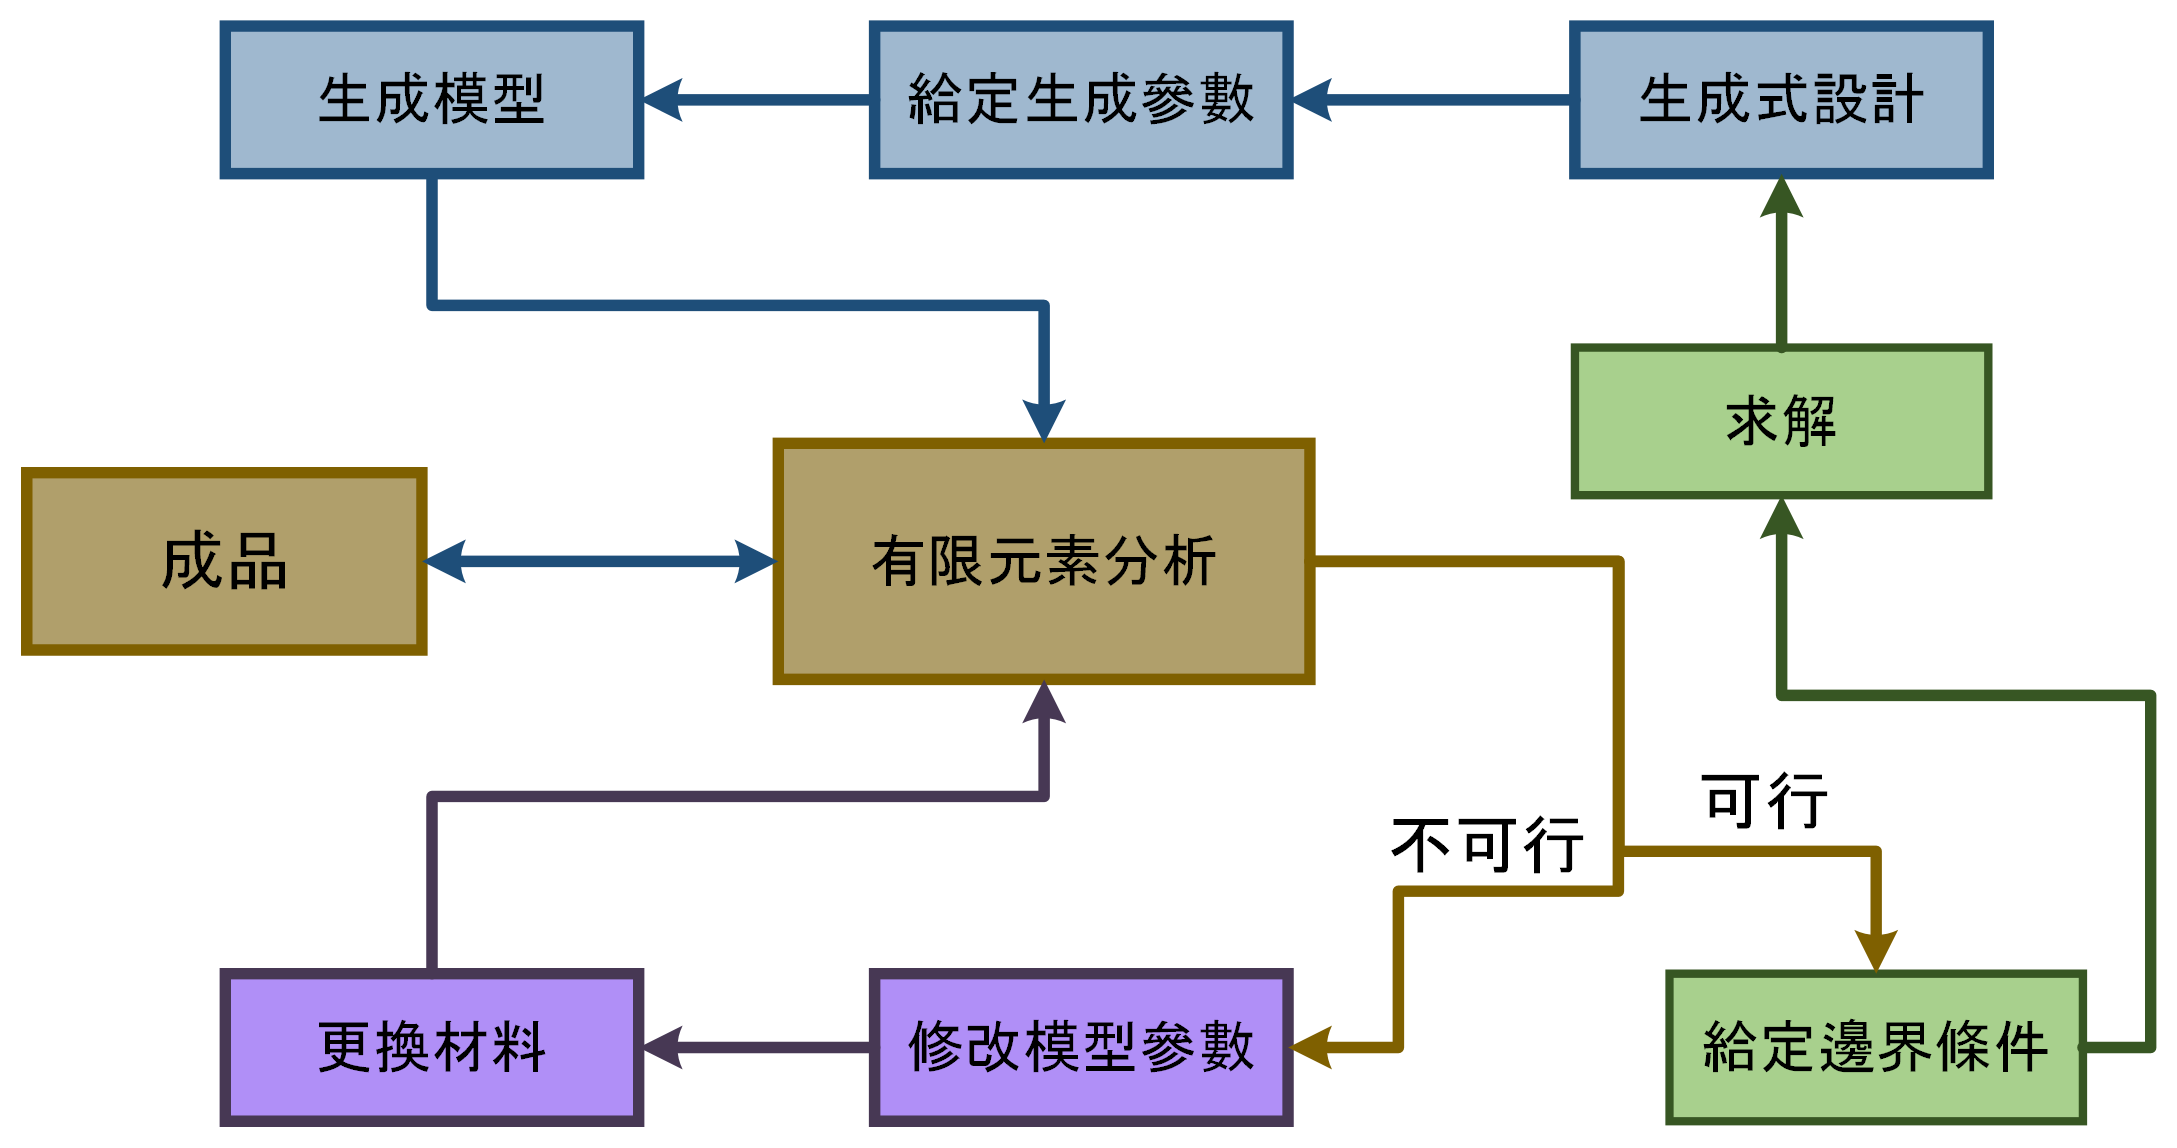
\includegraphics[width=10cm]{生成式流程}
\caption{\Large 生成式流程}
\label{生成式流程}
\end{figure}


主要依靠人工智能和機器學習來模仿自然界的進化設計方法,創造出許多種可能性,
利用AI運算生成整合並優化零件,創造出可能從未發現的幾何圖形,將產品創新優化,讓零件在輕盈的狀況下還保有堅韌程度,最大程度減低所需要耗費的人力、時間成本,讓成品可以快速並有效的產出。\\

%-----------------------生成式設計原理-------------------------%
\section{生成式設計原理}
生成式設計是一個迭代設計過程,透過軟體多次的分析與設計,生成符合製作條件的模型設計。生成式設計是一種電腦輔助設計的方法,利用軟體的AI智能算法,將設計者輸入的模型設計條件進行多次生成,並尋找出最佳設計。
生成式設計的主要功用為優化零件,不只能夠設計出更輕量化的零件,並且也能使各項性質提升,像是強度更強、更耐用、散熱快等。\\

%-----------------------設計流程-------------------------%
\section{設計流程}
\begin{itemize}
\item 定義問題:確定設計問題的範圍和目標
\item 創建設計規則:定義出用來生成設計方案的規則和條件。
\item	建立生成系統:選擇合適的軟體,利用AI生成設計。
\item 優化生成結果:當生成設計方案後,進行評估和優化,並對設計方案進行手動調整或修改,以便滿足特定的要求。\\

\end{itemize}

%-----------------------零件優化-------------------------%
\section{零件優化}
為了將零件輕量化,並維持其原本的零件強度,我們透過Solid Edge軟體將零件進行生成式設計,經過軟體的AI迭代算法以及多次修改設計參數,最後選擇最符合實際的設計。\

\begin{figure}[htbp]
  \centering
  \begin{minipage}{0.45\textwidth}
    \centering
    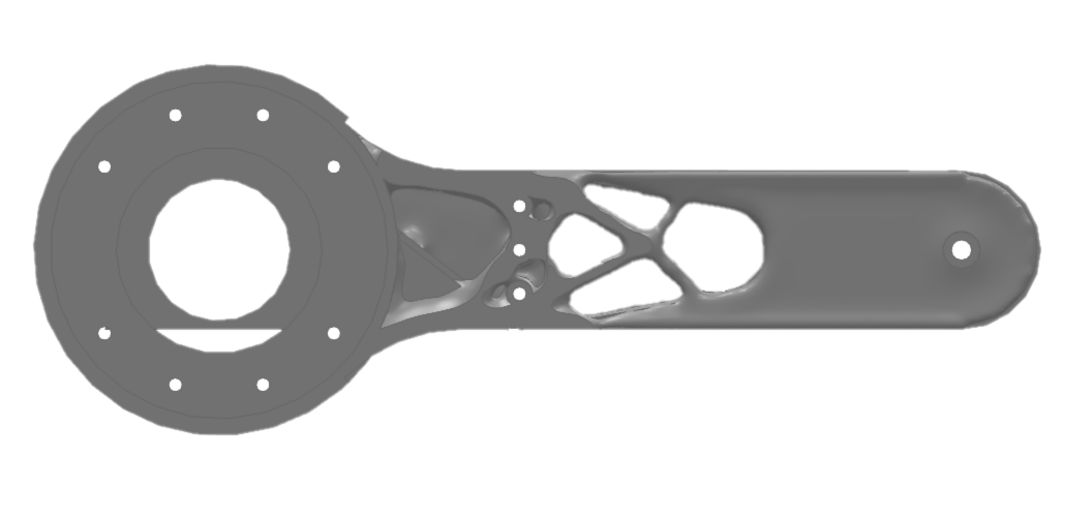
\includegraphics[width=\textwidth]{Leg1-1+1-5(拓樸)}
    \caption{Leg1-1+1-5(生成)}
    \label{Leg1-1+1-5(拓樸)}
  \end{minipage}
  \hfill
  \begin{minipage}{0.45\textwidth}
    \centering
    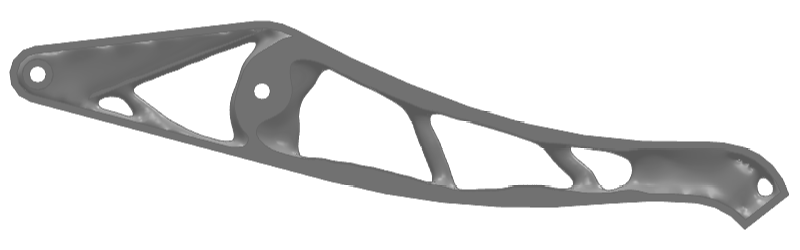
\includegraphics[width=\textwidth]{Leg4(拓樸)}
    \caption{Leg4(生成)}
    \label{Leg4(拓樸)}
  \end{minipage}
  \end{figure}

得到設計結果後,將原本的零件參考生成後的模型進行修改與挖空,這樣既保留所需的零件特徵,也達到了輕量化的目的,並使其外觀更加美觀。\

\begin{figure}[htbp]
  \centering
  \begin{minipage}{0.45\textwidth}
    \centering
    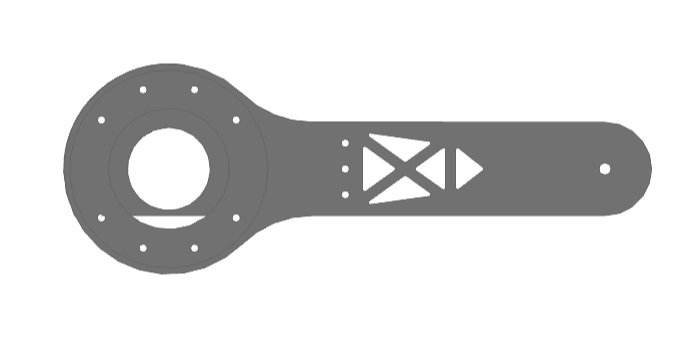
\includegraphics[width=\textwidth]{Leg1-1+1-5(輕量化)}
    \caption{Leg1-1+1-5(輕量化)}
    \label{Leg1-1+1-5(輕量化)}
  \end{minipage}
  \hfill
  \begin{minipage}{0.45\textwidth}
    \centering
    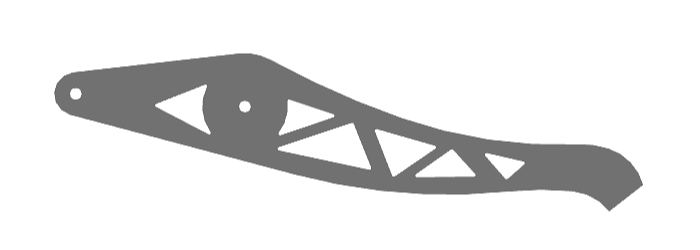
\includegraphics[width=\textwidth]{Leg4(輕量化)}
    \caption{Leg4(輕量化)}
    \label{Leg4(輕量化)}
  \end{minipage}
  \end{figure}

將零件輕量化後,必須確認這樣的修改方式是否與初始零件的數值相同或更加強壯,因此我們將初始零件和輕量化零件進行分析比對,以查證輕量化方式是否有誤。\

\begin{figure}[hbt!]
\center
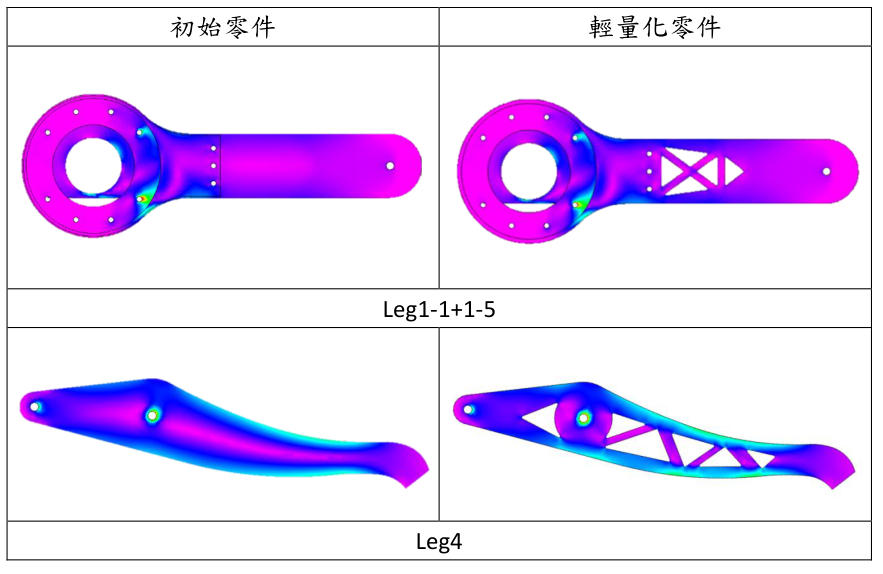
\includegraphics[width=16cm]{分析比對表(輕量化)}
\caption{\Large 分析比對表(輕量化)}
\label{分析比對表(輕量化)}
\end{figure}

\begin{table}[htb!]
  \center\large
  \setlength{\tabcolsep}{1cm}{
  \begin{tabular}{|c|c|c|}
    \hline   
    &最大應力(MPa)& 最小安全係數  \\
    \hline 
    初始零件&69.4 & 0.937 \\
    \hline 
    輕量化零件 &69.9& 0.929 \\
    \hline
  \end{tabular}}
  \caption{\Large leg1-1+1-5分析比對}
\end{table}

\begin{table}[htb!]
  \center\large
  \setlength{\tabcolsep}{1cm}{
  \begin{tabular}{|c|c|c|}
    \hline   
    &最大應力(MPa)& 最小安全係數  \\
    \hline 
    初始零件&61.2 & 1.06 \\
    \hline 
    輕量化零件 &60& 1.08 \\
    \hline
  \end{tabular}}
  \caption{\Large leg4分析比對}
\end{table}
\newpage
